%botanophobi2019haru-example.tex
% ABOUT: This is a very elementary example for the use of the beamer class
% inherited from upb2018.

\documentclass[handout]{beamer}

\usepackage[T1]{fontenc}
\usepackage[utf8]{inputenc}
\usepackage[english]{babel}

\usetheme[
		%blue 	% USTC blue
		%red	% Nature red
		green	% Nature Plants green
	,
		%oneslideonhandout		% one slide per page (landscape)
		%twoslidesonhandout		% two slides per page
		fourslidesonhandout		% four slides per page (landscape) [default]
]{bp2019haru}

% IMAGES
% chooose the cropped background image on the titlepage
\renewcommand{\titleimage}{logo/Background.JPG}
\renewcommand{\headerlogo}{logo/ustclonglogo.png}
\renewcommand{\framelogo}{logo/ustcshortlogo.png}

% GENERAL INFORMATIONS
\title[Gene Co-expression Network]{Botanophobia 2019 春\\这就是标题}
\subtitle{这是副标题}
\institute{生命科学学院}
\author{Student}
\date{Jan. 11st, 2019}

\begin{document}

% titlepage
\begin{frame}[plain]
	\titlepage
\end{frame}

\begin{frame}{Some TFs in \emph{Arabidopsis} have been identified}
	\begin{tabular}{lllll}
		\hline			
		AGI & TF & Regulate RSA & Study \\
		\hline
		AT2G14210 & ANR1 & yes & Zhang \& Forde, Science, 1998  \\
		AT5G67420 & LBD37 & - & Rubin et al, Plant Cell, 2009 \\
		AT3G49940 & LBD38 & - & Rubin et al, Plant Cell, 2009 \\
		AT4G37540 & LBD39 & - & Rubin et al, Plant Cell, 2009\\
		AT2G42200 & SPL9 & - & Krouk et al, Genome Biology, 2010 \\
		AT5G37020 & ARF8 & yes & Gifford et al, PNAS, 2008  \\
		AT4G24020 & NLP7 & yes & Castaings et al, The Plant Journal, 2009 \\
		AT5G49450 & BZIP1 & - & Obertello et al, BMC Systems Biology, 2010 \\
		AT1G64530 & NLP6 & - & Konishi \& Yanagisawa, Nature communications, 2014 \\
		AT5G07680 & NAC4 & yes & Vidal 2011 et al\\
		\hline  
	  \end{tabular}
\end{frame}

\begin{frame}{CO\textsubscript{2} Regulation of Stomatal}
	Ball-Berry-Leuning model
	$$g_{s} = g_{0} + \frac{_{1}A_{n}}{(c_{s}-\Gamma)(1+\frac{D_{s}}{D_{0}})}$$
	CO\textsubscript{2} signaling pathway in stomatal movement
	\vfill
	\begin{tikzpicture}
		\tikzset{>=latex}
		\node[inner sep = 0mm, align = flush left] (highCO2) at (0,0){High CO\textsubscript{2}};
		\node[inner sep = 0mm, align = flush left] (CA) at (3,0) {CA1/CA4};
		\node[inner sep = 0mm, align = flush left] (HCO3) at (5.5,0) {HCO\textsubscript{3}\textsuperscript{-}/RHC1}; 
		\node[inner sep = 0mm, align = flush left] (HT1) at (8,0) {HT1}; 
		\node[inner sep = 0mm, align = flush left] (ABA) at (3,-1) {ABA};
		\node[inner sep = 0mm, align = flush left] (1) at (4,-1) {};
		\node[inner sep = 0mm, align = flush left] (2) at (5,-1) {};
		\node[inner sep = 0mm, align = flush left] (3) at (6,-1) {};
		\node[inner sep = 0mm, align = flush left] (4) at (7,-0.3) {};	
		\node[inner sep = 0mm, align = flush left] (OST1) at (7,-1) {OST1};
		\node[inner sep = 0mm, align = flush left] (ca) at (7,-2) {Ca\textsuperscript{2+}};
		\node[inner sep = 0mm, align = flush left,color=\titlecolor] (sc) at (7,-3) {Stomatal Closure};

		\draw[->, dashed, color = ustcblack, line width = 1] (highCO2) to[bend right] (ABA);
		\draw[->, color=ustcblack, , line width= 1] (highCO2) -- (CA);
		\draw[->, color=ustcblack, , line width= 1] (CA) -- (HCO3);
		\draw[->, color=ustcblack, line width= 1] (ABA) edge (1) (1) edge (2) (2) edge (3) (3) edge (OST1);
		\draw[->, color=ustcblack, , line width= 1] (HCO3) to[bend left] (OST1);	
		\draw[->, color=ustcblack, , line width= 1] (OST1) -- (ca);
		\draw[->, color=ustcblack, , line width= 1] (ca) -- (sc);
		\draw[-|, color=ustcblack, line width = 1] (HT1) -- (4);

	\end{tikzpicture}
\end{frame}

\begin{frame}{ABA Regulation of Stomatal}
	Tardieu‒Davies model
	$$g_{s} = g_{min} + (g_{max} − g_{min} )\exp( − [ABA]\beta \exp(\delta \Psi_{f}))$$

	\vfill

	\begin{columns}
		\begin{column}{.4\linewidth}
			\begin{figure}
				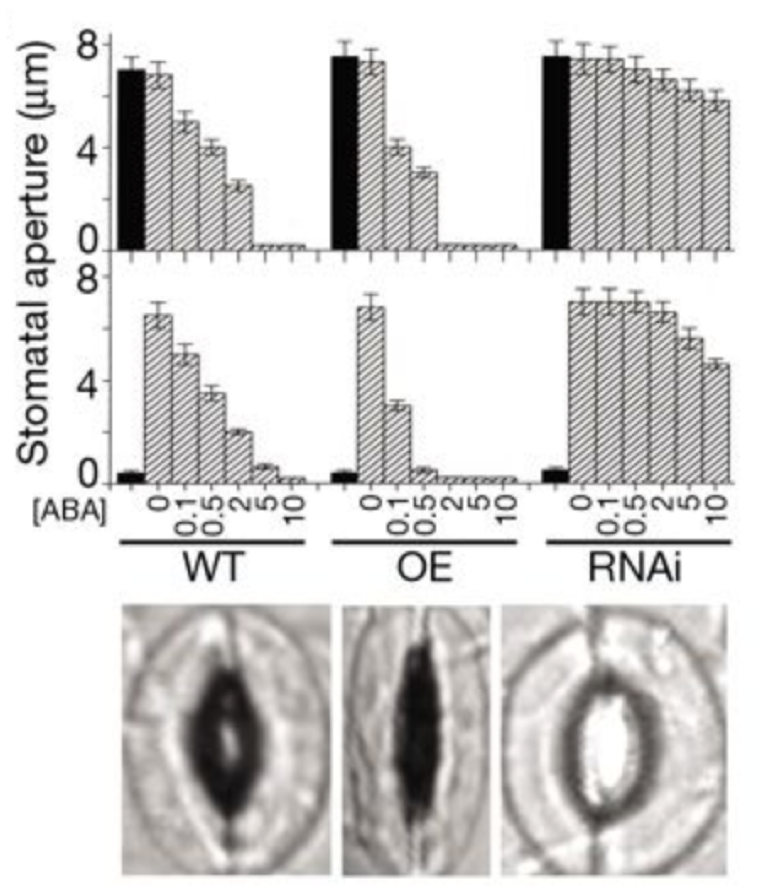
\includegraphics[width=.8\linewidth]{figure/figure1.png}
			\end{figure}
		\end{column}
		
		\begin{column}{.6\linewidth}
			\begin{figure}
				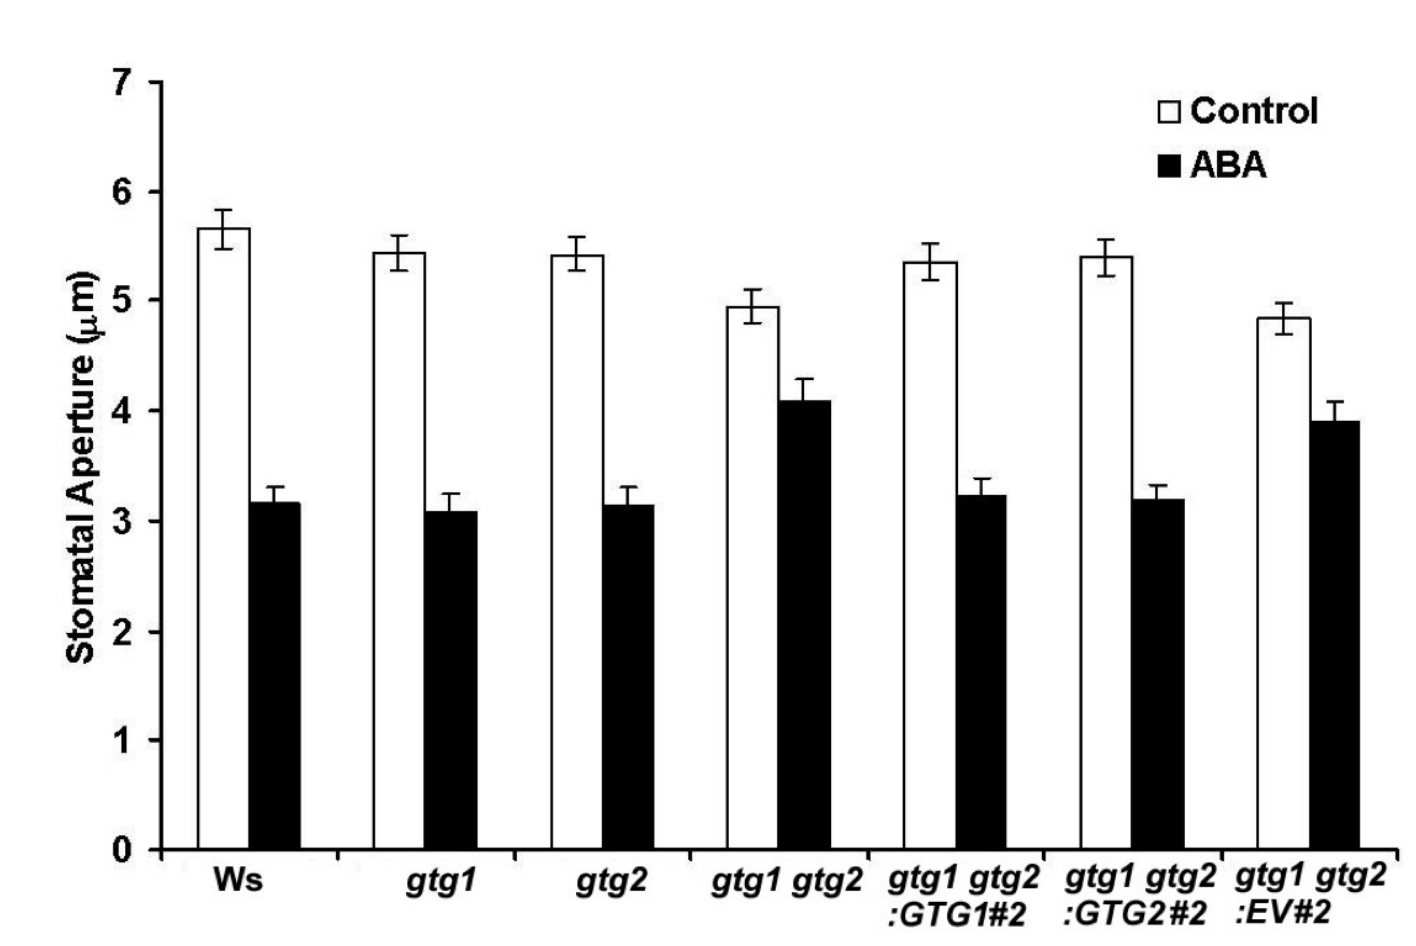
\includegraphics[width=\linewidth]{figure/figure2.png}
			\end{figure}
		\end{column}
	\end{columns}
\end{frame}


\end{document}
